\chapter{Implementation}\label{Chap:Implementation}

In this chapter I will write about some implementation aspects that were interesting or problematic during the development of the PARRHI system. For that, I will use a top down strategy, meaning, that I will talk about the general setup of the implemented system, and then drill down into the components. I will explain what software was used, why I made these decisions and whether or not they where good or bad in hindsight.

\section{PARRHI Hardware}
For the Augmented Reality purposes, I decided to use the first version of Microsoft's Augmented Reality glass called HoloLens~\cite{HoloLens}. The HoloLans has all needed capabilities like cameras for image and environment tracking, simple hand gesture recognition, a reasonably good field of view and was programmable with the 3D game engine Unity. Thankfully, the TUM chair of "Automation and Information Systems (AIS)" supplied me with this product.

The second main hardware component in the PARRHI system is the Robot. The robot manufacturing company Fanuc~\cite{Fanuc} was gracious enough to gift the TUM chair "Automation and Information Systems (AIS)" a free CR-7iA/L collaborative, 6 DOF, industrial robot~\cite{FanucCR7} and a R-30iB controller~\cite{FanucR30iB}. The R-30iB controller can either be programmed in Fanuc's TP-Language or in Fanuc's KAREL language. KAREL offers many possibilities with network sockets, reading and writing data from and to the robot's controller, whereas TP programmes are fit for moving and steering the robot.

The last component is a gripper provided by SCHUNK. The company gifted us a collaborative Co-act EGP-C~\cite{SchunkGripper}, that seamlessly integrated into the Fanuc robot with a hardware interface for exactly that purpose. 

At this point I would like to thank Fanuc, Schunk and the AIS massively for their supplies, so that this bachelor's thesis could be realised.

%4) Implementation
%- Introduction into the implementation, Main language
%4.1) PARRHI System and setup
\section{PARRHI Software}\label{Section:PARRHIHardware}
%- Generally: Some things in library, some things in Unity
Software Implementation wise, the PARRHI system is split up in three big components. First there is the PARRHI library, secondly the Robot library and lastly the Unity engine. The PARRHI library is the most intelligent component, since it contains all the logic for the Real World Model, the Parametrised Program, the Core Routine and commands the Input and Output Modules (see fig.~\ref{Fig:PARRHIConcept}). The Robot library has the tools necessary to communicate with the Robot in the Real World and is used by the Input and Output Modules. The third component \textit{Unity} hosts the PARRHI runtime library, and handles the AR-World, network communication etc.


\begin{figure}[!h]
	\centering
	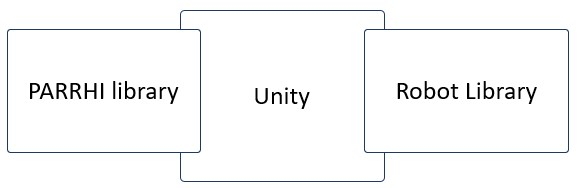
\includegraphics[width=0.5\textwidth]{Figures/Implementation_SystemSetup.jpg}
	\caption{PARRHI implementation setup}
	\label{Fig:Implementation}
\end{figure}


%4.2) PARRHI Library
\section{PARRHI Library}
%- Build up, workflow, interesting things
The PARRHI system was programmed in Microsoft's .NET framework version 4.6.1~\cite{NETFramework} using $C\#$ \cite{CSharp}. This decision was made because the Unity game engine is scripted in the language $C\#$. The PARRHI library itself is a \textit{Class Library} project~\cite{ClassLibrary} and has three main tasks.

\begin{enumerate}
	\item Import the Parametrised Program and perform some operations on it. The Parametrised Program is a XML~\cite{xmlW3C} based document. After importing, it is validated using an XSD~\cite{xsdW3C} document. Finally the PARRHI library has to extract useable $C\#$ objects from the deserialized XML document and setup references to resolve parameters.
	\item The Real World Model and the logic behind it is a subcomponent of this library. In my specific case, this means, that the PARRHI library contains the Robot's forward kinematics model and the required information to convert the HoloLens' internal coordinates, into the robot's coordinate system.
	\item The Core Routine is located in the PARRHI library, meaning, that on every iteration the PARRHI system calls into the PARRHI library to perform its task.
\end{enumerate}

This libraries main interface to the hosting environment or the caller is a container object, that contains all Parametrised Program object references like Holograms, Points etc., but also manages the importing of the Parametrised Program document itself. Fig.~\ref{Fig:ImplementationContainer} is a class diagram of the \code{Container} object. As it can be seen, it basically holds references to all objects of all types, and provides some update methods, that will be called from the library's host.

It is important to note, that all objects inherit from the \code{PProgramObject} class, which gives them the id property that allows the object to be identified. This is needed to resolve parameters in the Parametrised Program. As soon as an object is instantiated, it calls back to a list of id's which checks all ids for duplicates. In the case of duplicate ids, an error is thrown and displayed to the developer. Whenever an object is used as a parameter in the Parametrised Program, this id is used to find the reference to the target object.

\begin{figure}[!h]
	\centering
	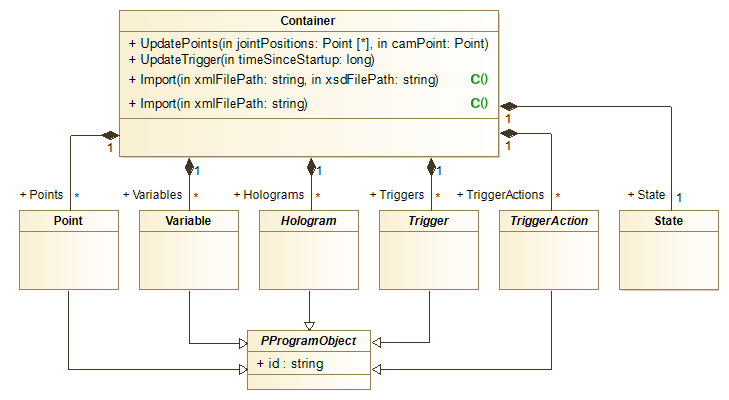
\includegraphics[width=1\linewidth]{Figures/Implementation_Container}
	\caption[Container Class Diagram]{Container Class Diagram}
	\label{Fig:ImplementationContainer}
\end{figure}

All compositions besides the \code{State} class simply represent the Parametrised Program objects presented in section~\ref{Section:ParametrisedProgram}. The \code{State} itself is an object, that holds the Real Worlds state data at all times, so that the PARRHI library has access to it. Fig.~\ref{Fig:ImplementationState} shows that the State object is composed of two other objects - each serving a specific purpose. The \code{Robot} class handles all operations that have anything to do with the robot. For example the Forward Kinematics. It also contains two delegates. Instead of letting the Robot class have an instance of the robot library (section~\ref{Section:RobotLibrary}), I chose to let this class have two delegates. The PARRHI library invokes these two delegates, which will be configured from the hosting environment. This creates some independence from the Robot Library, and may allow the PARRHI library to be used with absolutely any robot as long as there is a .NET framework controller for it.

This is not the only advantage of abstracting the controlling of the robot. During the development of the PARRHI system, I wanted to simulate as much as possible since I did not always have access to the robot. So I created an Interface between the PARRHI system and the real world, that was able to simulate all values instead of retrieving them from the real world. In the case of a simulation, I can then simply set this delegate to send the commands into the simulation, and not to the real robot.  

The \code{World} class has attributes that represent the state of the real world and discloses them to the PARRHI library. The \code{SetUIText} delegate similarly to the \code{MoveDelta} method from the \code{Robot} class, is a function pointer that can be configured from the library's host. This was done for the exact same reasons as with the \code{Robot} class - to create independence from the host.

\begin{figure}[!h]
	\centering
	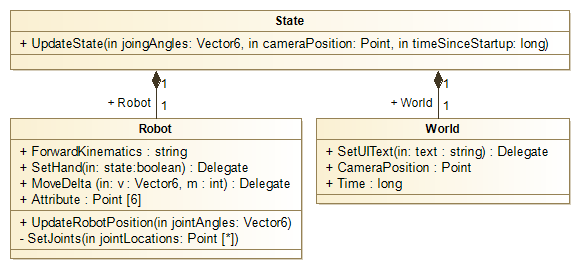
\includegraphics[width=0.7\linewidth]{Figures/Implementation_State}
	\caption[UML Class Diagram of State class]{UML Class Diagram of State class}
	\label{Fig:ImplementationState}
\end{figure}

These two classes are the main interface to the library's host. They contain multiple sub classes which will be explained in the following section.

\subsection{Parametrised Program objects}
The Parametrised Program contains five different objects: Variables, Points, Holograms, Triggers and Actions. During the implementation, I first created abstract classes of each object type, and then created concrete implementations for each sub-type. The PARRHI interpreter only utilises the public methods that are disclosed in the abstract classes. I chose this approach, because this way it is not important how the abstract class was instantiated, but only what values they hold.

This approach also allows the PARRHI system, to (for example) use any type of Point for the definition of a Hologram. The abstract Point class provides all data that is needed for the Hologram's definition. It is not important which concrete implementation the given instance is. This section will explain how these objects were implemented and how the inheritance tree is setup.

The Variable class is very straight forward and literally only contains an integer value, hence, it would be too much to draw a class diagram for it. There is also only one type of it, which makes it even simpler. 

The Point class on the other hand is a bit more interesting. The abstract Point class contains the 3 dimensional position vector, and some read-only properties, but the inheriting classes define how the position is set. For example the PointRobot class takes two joint indexes for its definition as it was described in section~\ref{Section:Points}. In each cycle, the public method UpdatePoint is invoked, which allows the PointRobot to calculate its new position. The \code{PointCamera} and \code{PointFix} do not add or overwrite any methods, since the \code{Point} class contains all needed functionalities.


\begin{figure}[!h]
	\begin{minipage}{0.65\textwidth}
		\centering
		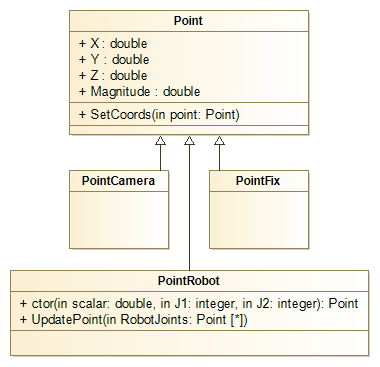
\includegraphics[width=0.8\linewidth]{Figures/Implementation_Points}
		\caption{UML Class Diagram of the Point class}
		\label{Ffig:ImplementationPoints}
	\end{minipage}\hfill
	\begin{minipage}{0.35\textwidth}
		\centering
		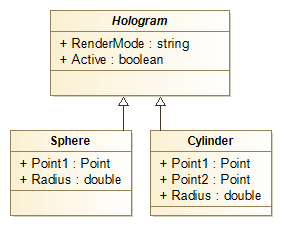
\includegraphics[width=1\linewidth]{Figures/Implementation_Holograms}
		\caption{UML Class Diagram of\\the Hologram class}
		\label{Fig:ImplementationHolograms}
	\end{minipage}
\end{figure}

The same principle was applied to the \code{Hologram} class~(see Fig.~\ref{Fig:ImplementationHolograms}). The two inheriting classes \code{Sphere} and \code{Cylinder} provide their specific constructors and hold their values. Since the \code{Point} instances in the two different Holograms are references to the real \code{Point} object, and the way references work, they do not have to be updated each cycle specifically. Only the hosting environment (in this specific case the Unity Game Engine) has to update the 3D objects it generates. 

The \code{Trigger} class~(Fig.~\ref{Fig:ImplementationTriggers}) is structured in a similar way.  The abstract class \code{Trigger} has a virtual method called \code{CheckTrigger}, which evaluates the trigger expression. Since every inheriting class triggers on different data, this method cannot be implemented in the parent class. As it was with the \code{Point} class, the different inheriting classes have different constructors, and store different data to evaluate their triggers. The \code{DistanceTrigger} for example takes two references to \code{Point} objects. It is important to note, that the Point object can be any object, that inherits from the \code{Point} class. This means, that the \code{DistanceTrigger} can be constructed with \code{PointCamera}, \code{PointRobot} or \code{PointFix}. Each inheriting class provides the \code{CheckTrigger} implementation, which corresponds to the defined boolean expression in section~\ref{Section:Events}.

\begin{figure}[!h]
	\centering
	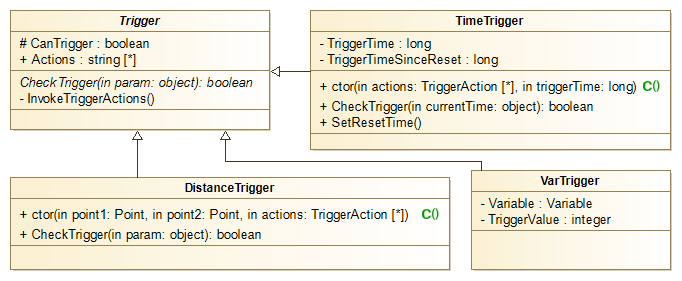
\includegraphics[width=0.7\linewidth]{Figures/Implementation_Triggers}
	\caption{UML Class Diagram of the Trigger class}
	\label{Fig:ImplementationTriggers}
\end{figure}

The last Parametrised Program object is the \code{Action} class. In this case, the abstract parent class is not as powerful as in the previous classes. The reason simply is, that all action types are fundamentally different and do not have anything in common, besides one method called \code{Action}. Figure~\ref{Fig:ImplementationAction} depicts the class structure here. Each inheriting class has to implement the virtual \code{Action()} method itself, since the parent object does not have the necessary data.

There are some interesting aspects to this implementation. As described, the \code{World} objects holds a function pointer (delegate) to a method, which prints a given string to the corresponding AR output. The \code{ChangeUITextAction} takes a reference to the \code{World::SetUIText(...)} delegate. This way, the hosting environment has to configure the UI delegate only once and it will be applied everywhere in the PARRHI library.

Similarly to the \code{ChangeUITextAction}, the \code{MoveRobotAction} holds a reference to the \code{Robot::MoveDelta(...)} delegate. In this specific case, the class has two different private attributes, which both save the position that should be sent to the robot. This is the case, because there are two different modes this Action can be used. In one case, the input can be a reference to a \code{Point} object and in the other case a six dimensional \code{Vector6} object. Remember, that the used Fanuc Robot is six dimensional. Since \code{Point} objects are only three dimensional, the robot will then approach the coordinates of the \code{Point} object from above, with the gripper facing downwards. The predefined orientation provides the last needed three coordinates, which completes the command and makes it executable. If a \code{Vector6} object is given, then the command can be sent without adjustments.

\begin{figure}[!th]
	\centering
	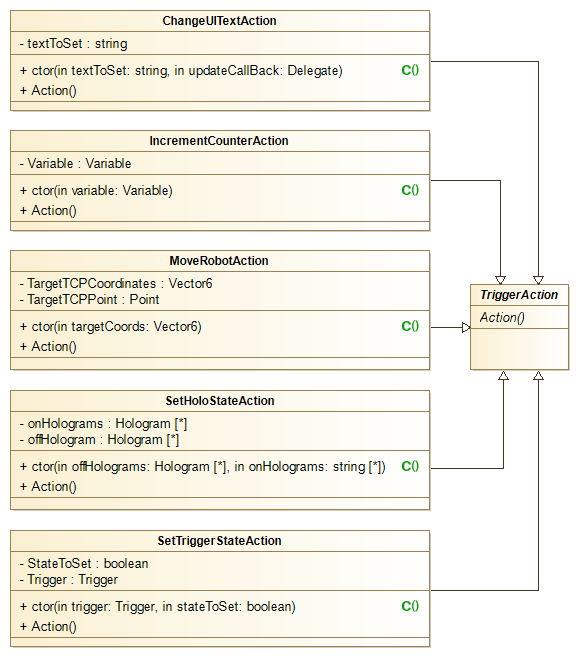
\includegraphics[width=0.7\linewidth]{Figures/Implementation_Action}
	\caption{UML Class Diagram of the Action class}
	\label{Fig:ImplementationAction}
\end{figure}

\subsection{Importing and interpretation of the Parametrised Program}
[This small subsection will describe how the xml is imported, how the needed information is extracted and how the described classes are instantiated - not yet finished, but will be quite short.]

Importing and validating the XML document is very easy, since the used .NET framework natively supports that. The implementation of the PARRHI Core Routine is also quite straight forward, which is why I will not talk about it too much. More interesting is the Robot's forwards kinematics, which will be presented now.

\subsection{CR-i7A Forward Kinematics}\label{Section:ForwardKinematics}
In robotics, a robot can be described in two different spaces. On one hand there is the joint space, meaning that all vectors and matrices depend on the joint positions, velocities or accelerations. Since the robot has six joints, the joint space is six dimensional. In the joint space the position vector is often represented as $ \vec{q} $.

On the other hand there is the task-space. In this space, all vectors and matrices depend on the Cartesian position and orientation (and their first two derivations) $ \vec{x}, \dot{\vec{x}}, \ddot{\vec{x}} $ of the robot's TCP. If the joint space is six dimensional, then generally speaking (ignoring cases like singularities) the task space is also six dimensional and represented as follows, with $x,y,z$ being the 3D coordinates, and $\alpha, \beta, \gamma $ being the orientation of the tip.
\[ \vec{q} = \begin{pmatrix} q_1 \\ q_2 \\ q_3 \\ q_4 \\ q_5 \\ q_6 \end{pmatrix}, \vec{x} = \begin{pmatrix} x \\ y \\ z \\ \alpha \\ \beta \\ \gamma \\ \end{pmatrix} with~~\vec{x},\vec{q} \in \mathbb{R}^6  \]

The forward kinematics now describes the process of transitioning form $ \vec{q} $ to $ \vec{x} $. This is done as follows: $ \vec{x} = f(\vec{q})~with~f: \mathbb{R}^6 \rightarrow \mathbb{R}^6$. Where the mapping $f$ depends on the robot's specific configuration and geometric properties. For reference, if $f$ is a mapping from $\mathbb{R}^6 \rightarrow \mathbb{R}^6$ then $f^{-1}$ (if it exists!) with $ \vec{q} = f^{-1}(\vec{x})$ is called inverse kinematics. 

To calculate $f$, I first defined local Cartesian coordinate systems after each joint. In fig.~\ref{Fig:ForwardKinematics} the green axes represent the robot, the black vector packs of three represent the coordinate systems $\phi_i = (x_i, y_i, z_i)$ and $\vec{l}_i$ represent the axes defined in the coordinate system $\phi_i$. In the following paragraph, the notation of  $\vec{l}_{a,b}$ will be used to name the $a^{th}$ vector called $\vec{l}$ expressed in the coordinate system $b$.

\begin{figure}[!h]
	\begin{minipage}{0.45\textwidth}
		\centering
		
\tdplotsetmaincoords{60}{120} 
\begin{tikzpicture}  [scale=0.08, tdplot_main_coords, axis/.style={->, black, thin}, 
vector/.style={-stealth,green,very thick}, 
robot/.style={green, very thick},
vector guide/.style={dashed,gray,thin}]

\usetikzlibrary{calc}

%standard tikz coordinate definition using x, y, z coords
\coordinate (O) at (0,0,0);

%tikz-3dplot coordinate definition using x, y, z coords


\pgfmathsetmacro{\axSize}{100}
\pgfmathsetmacro{\saxSize}{10}
\pgfmathsetmacro{\jointRadius}{30}

%Robot Points in cm (mm too large dimensions for library)
\coordinate (P0) at (0,0,0);
\coordinate (P1) at (5,0,33);
\coordinate (P2) at (5, 0, 77);
\coordinate (P25) at (10, 0, 100.5);
\coordinate (P3) at (15, 0, 100.5);
\coordinate (P4) at (47, 0, 100.5);
\coordinate (P5) at (55, 0, 100.5);
\coordinate (P6) at (63, 0, 100.5);


%draw coordinate system axes
%\draw[axis] (0,0,0) -- (\axSize,0,0) node[anchor=north east]{$x$};
%\draw[axis] (0,0,0) -- (0,\axSize,0) node[anchor=north west]{$y$};
%\draw[axis] (0,0,0) -- (0,0,\axSize) node[anchor=south]{$z$};


\draw[axis] (P0) -- (\saxSize,0,0) node[anchor=north east]{$x_0$};
\draw[axis] (P0) -- (0,\saxSize,0) node[anchor=north west]{$y_0$};
\draw[axis] (P0) -- (0,0,\saxSize) node[anchor=west]{$z_0$};

\draw[axis] (P1) -- ($ (P1) + (\saxSize,0,0)$) node[anchor=north east]{$x_1$};
\draw[axis] (P1) -- ($ (P1) + (0,\saxSize,0)$) node[anchor=north west]{$y_1$};
\draw[axis] (P1) -- ($ (P1) + (0,0,\saxSize)$) node[anchor=west]{$z_1$};

\draw[axis] (P2) -- ($ (P2) + (\saxSize,0,0)$) node[anchor=north east]{$x_2$};
\draw[axis] (P2) -- ($ (P2) + (0,\saxSize,0)$) node[anchor=north]{$y_2$};
\draw[axis] (P2) -- ($ (P2) + (0,0,\saxSize)$) node[anchor=south]{$z_2$};

\draw[axis] (P3) -- ($ (P3) + (\saxSize,0,0)$) node[anchor=south east]{$x_3$};
\draw[axis] (P3) -- ($ (P3) + (0,\saxSize,0)$) node[anchor=north west]{$y_3$};
\draw[axis] (P3) -- ($ (P3) + (0,0,\saxSize)$) node[anchor=south]{$z_3$};

\draw[axis] (P4) -- ($ (P4) + (\saxSize,0,0)$) node[anchor=south east]{$x_4$};
\draw[axis] (P4) -- ($ (P4) + (0,\saxSize,0)$) node[anchor=south west]{$y_4$};
\draw[axis] (P4) -- ($ (P4) + (0,0,\saxSize)$) node[anchor=south]{$z_4$};

\draw[axis] (P5) -- ($ (P5) + (\saxSize,0,0)$) node[anchor=north east]{$x_5$};
\draw[axis] (P5) -- ($ (P5) + (0,\saxSize,0)$) node[anchor=north east]{$y_5$};
\draw[axis] (P5) -- ($ (P5) + (0,0,\saxSize)$) node[anchor=south]{$z_5$};

%draw the robot's joints and axes
\draw[robot] (P0) -- (P1); \fill[fill=gray] (P0) circle (\jointRadius pt);
\draw[robot] (P1) -- (P2); \fill[fill=gray] (P1) circle (\jointRadius pt);
\draw[robot] (P2) -- (P25); \fill[fill=gray] (P2) circle (\jointRadius pt);
\draw[robot] (P25) -- (P3); 
\draw[robot] (P3) -- (P4); \fill[fill=gray] (P3) circle (\jointRadius pt);
\draw[robot] (P4) -- (P5); \fill[fill=gray] (P4) circle (\jointRadius pt);
\draw[robot] (P5) -- (P6); \fill[fill=gray] (P5) circle (\jointRadius pt);

%draw the 
\node[tdplot_main_coords,anchor=east] at ($(P0) + (10,0,15)$){$\vec{l_0}$};
\node[tdplot_main_coords,anchor=east] at ($(P1) + (5,0,20)$){$\vec{l_1}$};
\node[tdplot_main_coords,anchor=east] at ($(P2) + (-12,0,00)$){$\vec{l_2}$};
\node[tdplot_main_coords,anchor=east] at ($(P3) + (10,0,10)$){$\vec{l_3}$};
\node[tdplot_main_coords,anchor=south east] at ($(P4) + (-1,1,0)$){$\vec{l_4}$};
\node[tdplot_main_coords,anchor=north] at ($(P5) + (0,0,0)$){$\vec{l_5}$};




\end{tikzpicture}
		\caption{Robot forward kinematics\\coordinate systems}
		\label{Fig:ForwardKinematics}
	\end{minipage}\hfill
	\begin{minipage}{0.45\textwidth}
		The matrix ($\phi_{n+1}$) allows the conversion from vectors expressed in the coordinate system $n + 1$ to the expression in system $n$, with $\vec{l}_{n+1,n} = \phi_{n+1}(q_{n+1}) * \vec{l}_{n+1,n+1}$. After transforming the vector $\vec{l}_{n+1}$ one can add the vector $\vec{l}_{n,n}$ because they are both defined in the same coordinate system. Meaning, that the position of the tip of the vector $\vec{l}_{n+1}$ relative to the origin of the coordinate system $n$ is, $\vec{x}_{n+1,n} = \phi_{n+1}(q_{n+1}) * \vec{l}_{n+1,n+1} + \vec{l}_{n,n} $.\\
		Repeating this process from $n = 5$ to $n = 0$, results in the robot's TCP position relative to the coordinate system $\vec{O}$, which is what we wanted. One has to remember, that only the matrices $\phi_{i}$ are variables, since they depend on $q_i$. The vectors $\vec{l}_i$ are constants. This means, that for each iteration one only has to calculate all matrices $\phi_i$ and can then calculate the positions $(x_i, y_i, z_i)$ of each coordinate system relative to the base system $\vec{O}$.
	\end{minipage}
\end{figure}

\FloatBarrier

Since the $C\#$ implementation of this algorithm is only about 20 lines of code (excluding the definitions of the matrices $\phi_i$ and the vectors $\vec{l}_i$), takes only about 4ns to run, and the end results are all joint positions in Cartesian coordinates relative to a base system, I am quite happy with the outcome. If one wanted to add multiple robots into this framework, it could be done quite easily by adding one additional world-coordinate system, where all robot base systems are embedded into.
	
Adjusting this model to other types of robots would be easy. If the adjusted joints are all 1 DOF and rotational, then only the rotation matrix $\phi_i$ has to be adjusted, and $\vec{l}_i$ still stays constant. If one included translational, linear joints, the vector $\vec{l}_i$ would depend on some variable, but the mathematical process would stay the same.

Implementation wise one interesting fact is, that Unity (the game engine which hosts the PARRHI library) uses a left-hand coordinate system, whereas my robot forward kinematics was done in a right handed system since that is how I learned it the past few years. This means, that the last step in the forward kinematics is, to transform all produced vectors into Unity's coordinate system, which is rather easy. I only needed to swap the $z$ and $y$ coordinates of each joint position.

For further reading into this topic see~\cite{murray2017mathematical}.
	
%4.3) Unity structure
\section{Unity}
%- What is unity?
Unity is the host of the PARRHI and Robot libraries. Originally, Unity itself is a game engine that helps developers to develop, publish, maintain and market their games~\cite{Unity}. Within recent years the company behind Unity, called Unity Technologies, made efforts to become a de facto standard for AR and VR development.

There are a lot of third party products for Unity that help the developer with image tracking and general AR interaction. The next paragraphs explain what libraries, and tools where used to handle hand gesture recognition and image tracking.

%4.3.1) General Setup
%\subsection{General Unity Setup}
%- How is library implemented


%4.3.2) Image Tracking
\subsection{Image Tracking}\label{Section:ImageTracking}
%- Vuforia Engine
For Image Tacking I used the Vuforia Engine~\cite{Vuforia}. This engine had a rather simple setup in Unity and worked relatively seamlessly in Unity. Compared to other engines and libraries the Vuforia Engine first of all worked, had a good documentation and a user friendly configuration. An important aspect is, that for non-commercial use it is free of charge. 

The PARRHI implementation makes use of two image markers. One of them is attached directly at the robot's base and is of course used to synchronise the Real World with the majority of the AR World. Since the centre of origin of the robot was not at its base, but about 30 cm above the first joint, there is a small translation between the image markers position and the AR World's coordinate system. The second image marker is used to display the User's UI. The User is given a small sheet of paper with the said image on it, and the PARRHI system projects the User's tasks, some configuration and debug options onto it.


%4.3.3) ARToolkit%
\subsection{AR-Toolkit}
%- AR Toolkit explanation and usage
Interacting with Augmented Reality objects is an essential part of AR environments. Fortunately, Microsoft's open sourced Mixed Reality Toolkit~\cite{MicrosoftMRToolkit} makes this an easy task. The library directly integrates into the Unity environment and allows easy hand gesture recognition (pinching) for clicking and pointing at objects in the augmented space. Since both the HoloLens and the Mixed Reality Toolkit are developed by Microsoft, the library utilises all features and allows for an easy integration.


%4.4) Robot Protocol
\section{Robot Library}\label{Section:RobotLibrary}
%- Strucutre, languages, problems, solutions
Next to the PARRHI library and Unity, the Robot library is the big third component in the PARRHI implementation. The following chapter will explain how we accessed the controller's data, transferred the data to the HoloLens and generally communicated with the robot. The whole Robot library was built together with Florian Leitner, who is currently writing his bachelor's thesis about a virtual programming environment of industrial robots at the same chair as I am. Since his thesis is being written at this very moment, I cannot reference to any source of his.

The Robot Library is responsible for the communication between any system that is capable of executing .NET framework applications, and the robot's controller R-30iB~(see section~\ref{Section:PARRHIHardware}). It is important to know, that Fanuc's controllers are not easily controllable by non-Fanuc components. Our goal was, to wirelessly control the robot from external devices that run .NET framework applications. Since there where no "plug and play" solutions available, we came up with the system, that will be explained in the rest of this chapter. As it has been done in the concept chapter, I will first shortly explain each component before elaborating on the information flow between them. Finally, I will give some details about the implemented, custom protocol we use. Fig.~\ref{Fig:RobotArchitecture} depicts how the system is actually setup.

\subsection{Robot Communication Architecture}

The architecture can be split up into nine individual components, ranging from the actual commanding application to the robot itself. This architecture is tightly linked with the concept of the PARRHI system, thus many components can be recognised.

\begin{figure}
	\centering
	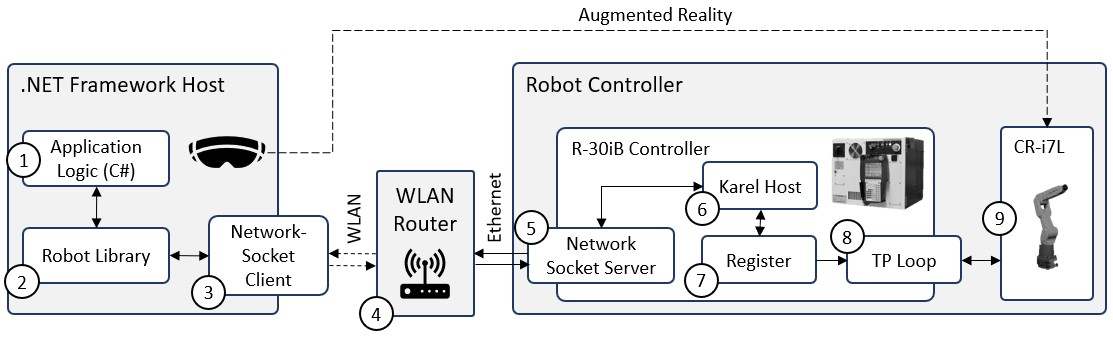
\includegraphics[width=1\textwidth]{Figures/RobotArchitecture.jpg}
	\caption{Robot library setup}
	\label{Fig:RobotArchitecture}
\end{figure}



\begin{enumerate}
	\item Application Logic: This is any application that wants to communicate with the robot. In my case the PARRHI system.
	\item Robot Library: A custom library written in $C\#$ that offers some wrappers around our custom protocol, which simply is a syntax we defined to transfer commands and data over the Network Socket. This protocol follows certain rules, so that both the KAREL Host and the $C\#$ Library can parse them to extract the important information in a standardised way.
	\item Network Socket Client: Standard Network Socket, where the PARRHI library represents the client.
	\item WLAN Router: Standard WLAN Router, which is connected to the controller via a standard patch cord.
	\item Network Socket Server: Standard Network Socket, where the R30iB controller represents the server.
	\item KAREL Host: A programm written in KAREL~\cite{FanucKarel} that receives commands from the network socket, parses them according to the defined protocol and returns the requested data or executes the requested commands.
	\item Register: A storage that is used to command the Teach Pendant (TP) Loop (8), which also has access to this storage location. Some registers are used to set different modes like coordinate systems, absolute versus relative and so on, and six registers are used to transfer vectors, that the TP program should process according to the set mode.
	\item TP Loop: A program written in TP that scans the Register (7) every cycle, and controls the robot accordingly.
\end{enumerate}

One can now see, that Application Logic (1) is the PARRHI itself. The network socket client(3) is the concrete implementation PARRHI's the in and output module and the complete Robot Controller is the "real world" excluding the end user.


Since researching the difference between KAREL and TP programmes on the internet is rather hard, because one simply does not find a lot of information about it, I would like to summarise our current knowledge about that. KAREL is a programming language, that is similar to Fortran. It was developed by Fanuc itself, and is used internally for a lot of components in the controller. Nowadays, KAREL is most often used for managing tasks like communication, synchronisation, data handling and so on. Teach pendant programmes on the other hand, are specialised on actually commanding the robot's movement and behaviour. TP supports numerous methods to control a robot, that the KAREL language simply does not offer. This is why, we chose to split up the controller-side software in these two programming components.


Now the information flow is as follows: First, the application (1), which wants to send a command to the robot has to call into the Robot Library (2). Besides managing the network socket connection (3), this library offers about 12 commands to the Application. A command could be the wish to fetch the robot's joint position, or to move the robot into a certain position. The Robot Library (2) then sends the command to the network socket (3), which is connected to the controllers server-endpoint. It is important, that the communication between the HoloLens (or a Laptop for instance) is wireless in order to stay mobile. The controller is connected to the WLAN Router (4) via a cable using the Ethernet protocol. There, the network socket server (5) receives the command, and passes it on to the KAREL Host (6). The latter then processes the command, which is described in the following section.

\subsection{Robot Communication KAREL Host}

At the point of reception, the command is only a string following a very specific syntax that we defined. The KAREL Host (6) then parses the command and acts on its instructions. If the command is a simple "Fetch Command", the KAREL Host (6) collects the needed data, constructs the message and sends it back via the network. If the command is targeted at the robot itself, the KAREL Host (6) fills the Register (7) with all necessary data that the TP Loop (8) needs to execute the movement command. This data is a six dimensional vector (coordinates in task or joint space), the mode whether the vector should be interpreted absolutely or relatively to the current position, the coordinate system which should be used to interpret the six dimensional data and some internal flags.

The KAREL code consists of four main parts. There is the network communication, the command parsing, the data collection/register writing and lastly the response sending. The KAREL language makes it relatively easy to parse strings and write the logic components that are needed for the communication system. We tried to achieve as much as possible within the KAREL Host, and limit the parallel running TP Program to its speciality, which is controlling the robot physically.

\subsection{Robot Communication TP Program}

The TP Loop (8) itself is written in Fanuc's TP-Language. It basically is one large loop, that reads the Register (7) and acts on its instructions. There are some problems that had to be overcome though. For example switching between the relative and absolute movement mode has one very critical aspect: During absolute movements, the values in the Register (7) might be relatively high, since the task space coordinates are defined in millimetres. Values here are in a range from -700 to +700 mm. When interpreting these coordinates absolutely, that is not a problem since they are in the robot's range of motion. But after switching to the relative mode, these values are added to the current robot position, resulting in a huge step, which most probably is not within the range of motion any more.

Another example here is the switching of coordinate systems. When the current data in the register was inserted to be interpreted as joint coordinates, the individual values are in the range from about -360° to +360° (varying for each joint). This range includes values close to zero. A limit error would occur, if these were to be interpreted as task space coordinates suddenly, since Cartesian positions close to zero are not possible in the task space. Cases like these have to be thought of and handled. 

Fig. \ref{Fig:TPLoopFlowChart} shows the TP Loop's Activity Diagram. Of course this is a rather simplified version, since almost every action depends on two register values, which represent the coordinate system and the relative/absolute mode. 

\begin{figure}
	\centering
	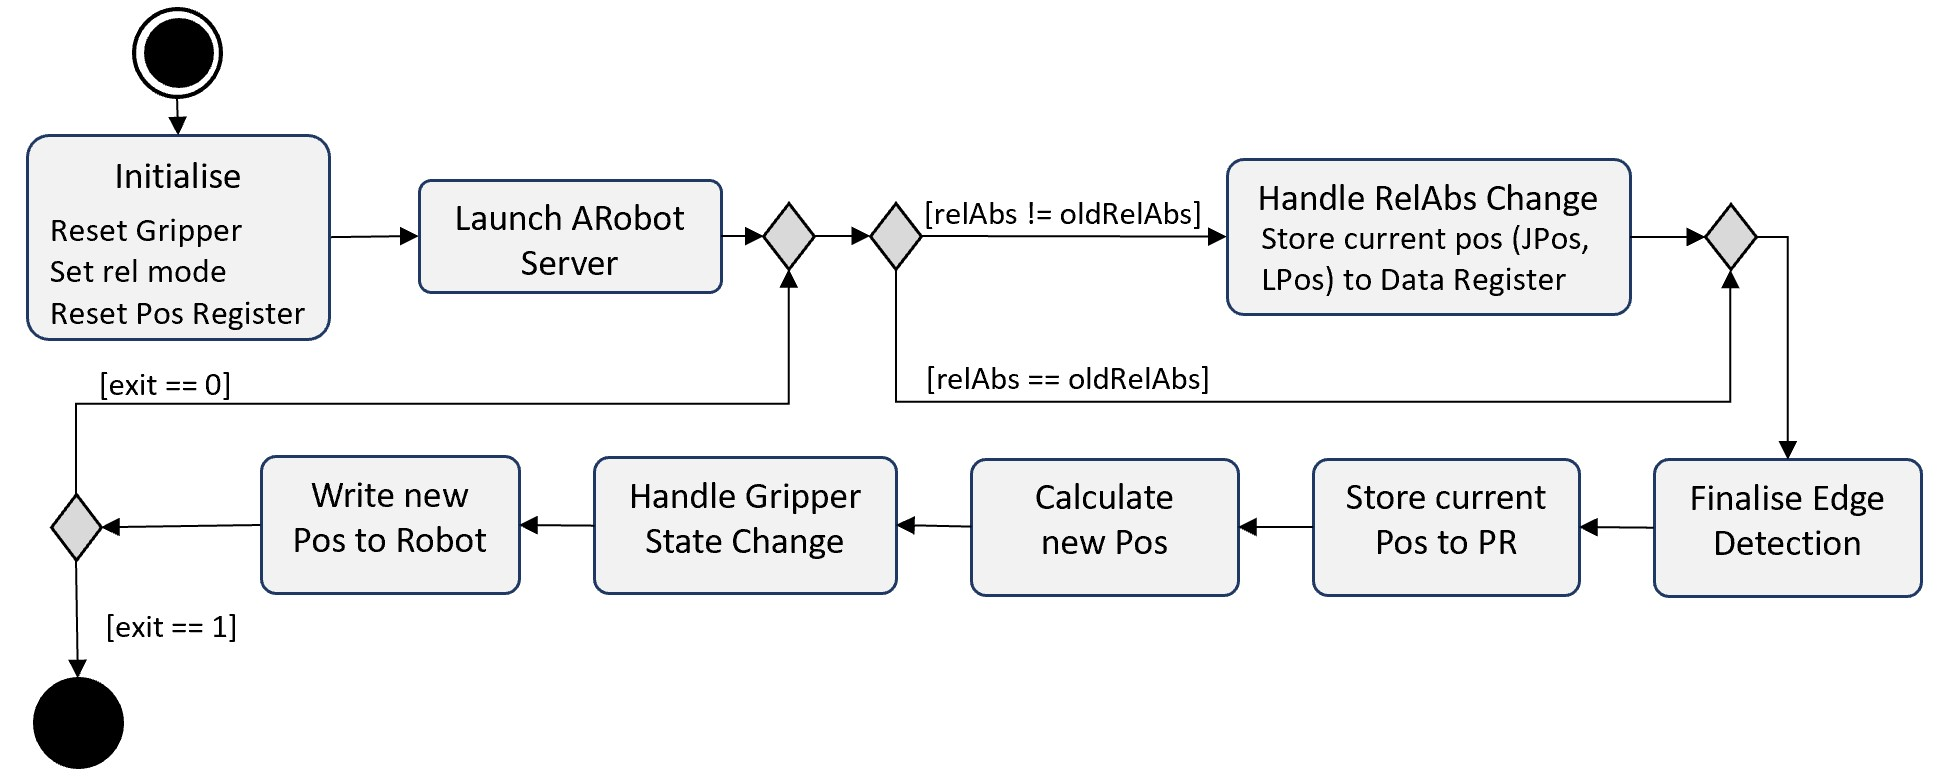
\includegraphics[width=0.9\linewidth]{Figures/TPLoopFlowChart.jpg}
	\caption{}
	\label{Fig:TPLoopFlowChart}
\end{figure}

Resetting the register's state at the very beginning is crucial, since the data registers are persistent stores, which means, that their value is saved even when the controller is shut down. The initialisation defines a clear behaviour at each launch of the program.

The \textit{Launch ARobot\_Server} action starts the KAREL Host, which communicates with any potential client via the network socket. After starting the KAREL Host, the program has to check if the relative/absolute mode has changed. If so, it handles this change to avoid unexpected behaviour due to old data in the registers. This is done via an edge detection, which needs an additional variable to store the previous mode. 

The action \textit{Store Current Pos to PR} fetches the current coordinate vector in the corresponding system (joint space or task space), which is then fed into the next action, which calculates the new target position vector. This action differentiates between the relative and absolute mode. 

After the hand gripper state change is set, the new target position is written to the robot - again within the corresponding coordinate system. At the very end there is an \textit{exit} flag, which can be set to \textit{'1'} by the KAREL Host. This quits the KAREL and TP Programm and thus allows the client (.NET library) to send an exit command to the robot. This gives the controller an opportunity to safely shutdown the network socket and the TP Loop. 

\subsection{Robot Motion Group Management}

One important aspect to mention is the motion control system, which all FANUC robots are subject to. Within the FANUC environment, the robot can be separated into motion groups, which are groups of moveable elements within a FANUC robot. One motion group may for example contain the first three joints, and another motion group could own the second three joints. Or, one group can also contain all joints. At runtime, a motion group can be physically controlled by only one instance at at time. TP programmes, KAREL programmes and also the Teach Pendant are viewed as instances here. The reason for this is, to avoid cases, where undefined behaviour through double commanding might occur. 

Since applications, which were developed in the PARRHI system, should both allow the user to jog the robot and then take over control programmatically through actions, the right to move the robot has to be managed. In this case there are two involved instances: The Teach Pendant and the TP Loop program.

The solution to this problem was, to implement a motion group control ownership management system. By default, the TP Loop would release the motion group control and not be able to move the robot, unless it really needs to execute a corresponding command. This means, that unless the TP Loop actively controls the robot, the Teach Pendant has the ownership over the motion group, so that the user can jog the robot.

Implementation wise, this was achieved by a "pause" flag in the data register. As soon as the KAREL program sets this pause flag to "1", the TP loop starts a second TP program called \textit{"Waiter"}, which does not have any motion control rights and then aborts its own execution - this actually releases the motion control. This waiter program simply waits until the pause flag gets reset to "0" by the KAREL program, and then restarts the TP loop. While the waiter program waits, the motion control rights are owned by the Teach Pendant, and thereby the user can take control over the robot. As soon as the PARRHI system has to control the robot, it activates the TP loop by setting the pause flag to "0", executes its movement command and then releases the motion control by setting the pause flag to "1".

\subsection{Robot Communication Outcome}

Basically, the presented architecture allows us to execute any pre-defined function in a fraction of a second. The whole process is actually so fast, that the PARRHI system fetches the robot's joint position in each iteration.

To finish this chapter off, I would like to shortly explain what the system is capable of doing. The Robot Library can get the robot's joint angles, TCP position and six dimensional force/torque sensor data. It can command the robot to drive to an absolute or relative task or joint space position and set a speed vector for the TCP and joint vector. Finally, there are commands that are mainly used internally at the moment, which release and claim the motion control. Generally, this system could be extended quite easily, by defining new commands in the robot library and the KAREL host.

%4.5) Parametrised Program Validation and Definition
\section{Parametrised Program Implementation and Validation}
One core component of the PARRHI implementation is the Parametrised Program. The document needs a hierarchical or at least well defined structure, since the content has to be imported (de-serialised). This automatic process only works seamlessly, if certain rules are kept perfectly. This is also why, it makes sense to validate the document before de-serialising it, since the PARRHI system has some presupposed assumptions about the document.  

XML~\cite{xmlW3C} seems to fulfil these requirements. XML documents are strictly hierarchically and have the big benefit of being human and machine readable. In PARRHI's case this is exactly what the document in question should be. Written by a human with possibly limited software engineering skills, but interpreted by a machine.


%4.4.1) XML Structure
\subsection{Parametrised Program XML Structure}
%%- Give XML Tags
The content of the Parametrised Program was thoroughly discussed in section~\ref{Section:ParametrisedProgram}. In this section, I would like to present the actual implementation and how a Parametrised Program written in XML would look like.

XML documents must have one root element. In PARRHI's case this is the "<PProgram/>" tag. Similarly to the conceptual train of thought, the actual implementation contains four children.

\begin{lstlisting}
<?xml version="1.0"?>
<PProgram xmlns="PARRHI">
	<Variables>...</Variables>
	<Points>...</Points>
	<Holograms>...</Holograms>
	<Events>
		<Trigger>...</Trigger>
		<Actions>...</Actions>
	</Events>
</PProgram>
\end{lstlisting}

Each child element of PProgram can now take their object definitions directly. Only the "Events" element categorises its content in two sub elements "Triggers" and "Actions". It is important to know, that every object defined in the Parametrised Program has to have a unique name attribute to identify it in other parts of the application. 

The following block of code exemplary defines each object once. Please note, that this program is not written to actually do something meaningful, it only presents all ways to define objects in the Parametrised Program. Of course the Developer could use every object multiple times and also create multiple instances of the same object types, as long as their name is unique.

\begin{lstlisting}
<?xml version="1.0"?>
<PProgram xmlns="PARRHI">
	<Variables>
		<Int name="Variable0">0</Int>
	</Variables>
	<Points>
		<PointCamera name="CamPoint"/>
		<PointFix name="FixPoint0" X="200" Y="-300" Z="300" />
		<PointRobot name="RobotPoint0" J1="1" J2="2" Scale="0.6" />
	</Points>
	<Holograms>
		<Cylinder name="Cyl0" point1="CamPoint" point2="FixPoint0" radius="10" visibility="hidden"/>
		<Sphere name="Sphere0" point="RobotPoint0" radius="25" renderMode="transparent" visibility="visible"/>
	</Holograms>
	<Events>
		<Trigger>
			<DistanceTrigger name="DistanceTrigger0" canTrigger='true' point1="CamPoint" point2="RobotPoint0" distance="15.5" actions="HoloStateAction0"/>
			<VarTrigger name="VariableTrigger0" canTrigger='true' varName="Variable0" triggerValue="2" actions="IncrVarAction0"/>
			<TimeTrigger name="TimeTrigger0" canTrigger='true' timeSinceActivation="120" actions="TriggerStateAction ChangeUITextAction0"/>
		</Trigger>
		<Actions>
			<IncrementCounterAction name="IncrVarAction0" intVar="Variable0"/>
			<SetHologramStateAction name="HoloStateAction0" onHolograms="Sphere1 Sphere2 Zyl2" offHolograms="Zyl1"/>
			<SetTriggerStateAction name="TriggerStateAction0" triggerName="Trigger1" canTrigger='true'/>
			<ChangeUITextAction name="ChangeUITextAction0" text="Tutorial step nr. 4"/>
			<MoveRobotAction name="MoveRobotAction0" target="100 100 100 45 15 0/>
			<SetRobotHandStateAction name="SetRobotHandAction0" state="open" />
		</Actions>
	</Events>
</PProgram>
\end{lstlisting}

It does not matter in which sequence all the elements occur. Only the hierarchically structure has to be kept exactly as the example document above. The PARRHI library will at some point deserialise the Parametrised Program using a standard .NET Framework XML library. For this deserialisation a validation should be performed, in order to find flaws beforehand.

%4.4.2) XSD generation and validation#
\subsection{XSD generation and validation}
%- Auto generate xsd and c# classes
The hierarchy of XML documents can be specified very detailed in XML-scheme documents, which are also called XSD files~\cite{xsdW3C}. These documents define which element can or must occur at witch location in the XML document, which attributes these elements can or must have and so on. The XSD file can even specify minimum and maximum values, data types and much more.

Hence, an XSD document is an essential part in the importing / validation process. Since writing these documents can be enormously work intensive, Microsoft has developed ways to generate XML schemes from a set of XML documents. Especially, when the underlying XML document may change repeatedly, it can be very exhausting to update the XSD file every time. For that I wrote a small $C\#$ application, that takes multiple .xml documents as an input, and outputs one XSD document that defines rules, which fit to all input XML files. 

Another application developed by Microsoft called "xsd.exe"~\cite{xsdExe} allows to convert XSD documents into $C\#$ class definitions. During the development of this bachelor's thesis, I automated the process of generating the XSD file and from that the $C\#$ class definition, using the programming language Perl~\cite{perl}.

This means, that whenever an attribute had to be added to some xml element in the Parametrised Program, this attribute had to be added in one of the example input xml documents and the execution of the Perl script would then output new XSD documents and a $C\#$ class to deserialise the Parametrised Program. 

One huge advantage of XSD documents and their validator is, that the latter can output exact error messages with what went wrong in the input xml document. This includes the type of error, line and column numbers, and (depending on the error type) suggests how to fix it. For the PARRHI system this means, that very exact feedback can be printed to the user if any errors occur. This makes it easier for non software engineers to accomplish their task.




















